\chapter{Ley de Gauss}

\begin{miparrafo}

En electromagnetismo el flujo eléctrico, o flujo electrostático, es una magnitud escalar que expresa una medida del campo eléctrico que atraviesa una determinada superficie, o expresado de otra forma, es la medida del número de líneas de campo eléctrico que penetran una superficie. Su cálculo para superficies cerradas se realiza aplicando la ley de Gauss. Por definición el flujo eléctrico parte de las cargas positivas y termina en las negativas, y en ausencia de las últimas termina en el infinito. 


El flujo eléctrico en unidades del Sistema Internacional (SI) se expresa en $\mathrm{V\ m}$, o, de forma equivalente, $\mathrm{N\ m}^2 \mathrm{C}^{-}1$ 


Faraday (s. XIX) supuso que existía un flujo eléctrico, y concluyó que era proporcional a la carga. Fue Carl Friedrich Gauss (s. XIX) quien expresó matemáticamente esta relación, dando lugar a la ley que lleva su nombre.


En física la ley de Gauss, relacionada con el Teorema de la divergencia o Teorema de Gauss, establece que el flujo de ciertos campos a través de una superficie cerrada es proporcional a la magnitud de las fuentes de dicho campo que hay en el interior de la misma superficie. Estos campos son aquellos cuya intensidad decrece como la distancia a la fuente al cuadrado. La constante de proporcionalidad depende del sistema de unidades empleado.
Se aplica al campo electrostático y al gravitatorio. Sus fuentes son la carga eléctrica y la masa, respectivamente. También puede aplicarse al campo magnetostático.

La ley fue formulada por Carl Friedrich Gauss en 1835, pero no fue publicado hasta 1867. Esta es una de las cuatro ecuaciones de Maxwell, que forman la base de electrodinámica clásica (las otras tres son la ley de Gauss para el magnetismo, la ley de Faraday de la inducción y la ley de Ampère con la corrección de Maxwell). La ley de Gauss puede ser utilizada para obtener la ley de Coulomb, y viceversa.

\end{miparrafo}

\section{Flujo de un campo vectorial}

\begin{multicols}{2}
Supóngase una región del espacio en que existe un campo vectorial $\vec V$ y sea $S$ una superficie arbitraria de esa región, en la cual, arbitrariamente, elegimos un sentido de recorrer su periferia.

Un elemento de superficie $\dd S$ lo representaremos por un vector $\overrightarrow{\dd S}=\dd S \vec u_N$, con $\vec u_N$ un vector unitario perpendicular a la superficie en el sentido de avance de un  sacacorchos al rotar en el sentido arbitrario que hemos escogido. 
\begin{figure}[H]
	\centering
	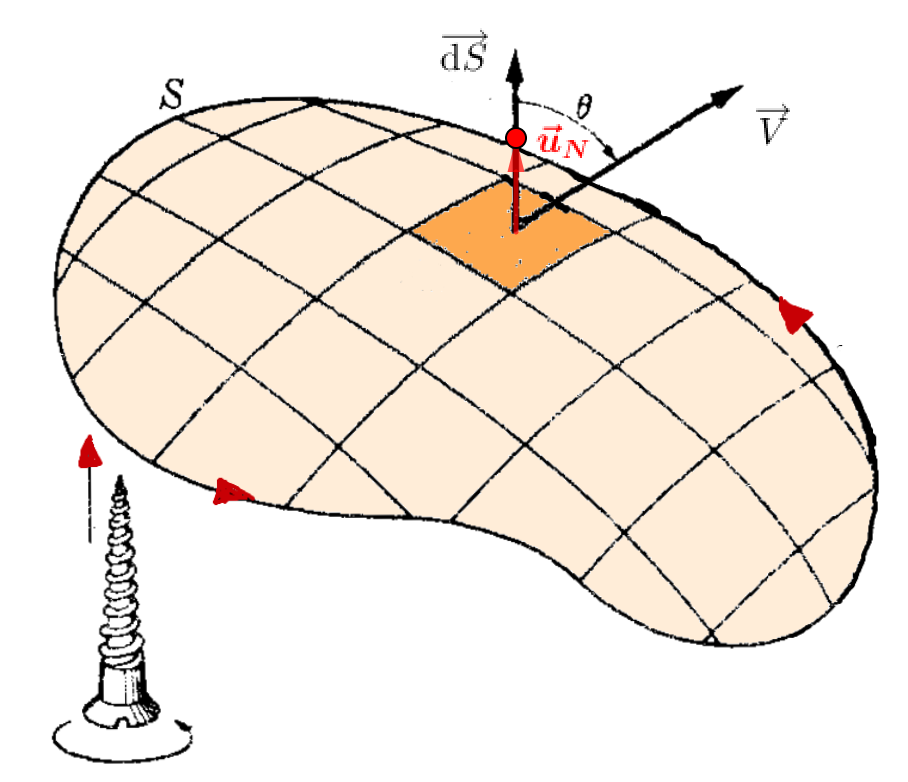
\includegraphics[width=.55\textwidth]{imagenes/imagenes23/T23IM01.png}
\end{figure}	
\end{multicols}

Por definición, recibe el nombre de 	\emph{flujo elemental vectorial}, $\dd \Phi$, al producto escalar del campo vectorial $V$ por el elemento diferencial de superficie $\dd \vec S$.

\begin{equation}
\subrayado{\ \boldsymbol{
\dd \Phi= \vec V \cdot \dd \vec S=\vec V \cdot \vec u_N \dd S= V \cos \theta \dd S} \ }
\end{equation}

Para calcular el flujo total que atraviesa la superficie $S$ integraremos a través de toda la superficie $S$.

\begin{equation}
\subrayado{\ \boldsymbol{ \Phi = \int_S \vec V \cdot \dd \vec S 	} \ }
\end{equation}

El flujo total puede ser positivo, negativo o nulo. Si es positivo $(0^o<\theta<90^o)$, se denomina ``saliente'', y si es negativo $(90^o<\theta<180^o)$, ``entrante''. Si la superficie es cerrada como una esfera o un elipsoide, se escribe un círculo sobre el signo integral.

\begin{equation}
	\Phi= \oint_S \vec V \cdot \dd \vec S 
\end{equation}


\begin{multicols}{2}
\small{El nombre de flujo se debe a su aplicación al estudio de los fluidos. Supongamos que tenemos un chorro de partículas, todas moviéndose hacia la derecha con velocidad $v$. Aquellas partículas que atraviesan la superficie $\dd S$ en el tiempo $t$ estarían contenidas en un cilindro de base $\dd S$, generatriz paralela a $v$ y longitud $vt$. Este volumen es $vt \dd S \cos \theta$. Suponiendo que haya $n$ partículas por unidad de volumen, el número total de partículas que pasa a través de la superficie $\dd S$ en el tiempo $t$ es $nv \dd S \cos \theta=n\vec v \cdot \vec u_n \dd S=n\vec v\cdot \dd \vec S$}, lo que concuerda formalmente con nuestra definición de flujo.\normalsize{.}
\begin{figure}[H]
	\centering
	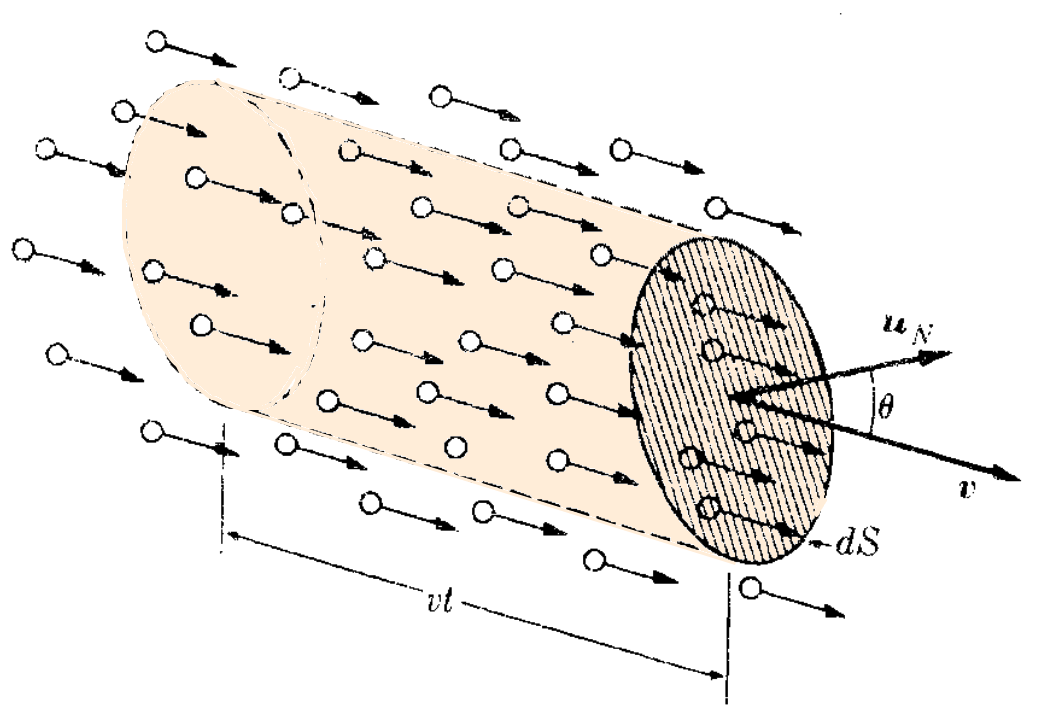
\includegraphics[width=.5\textwidth]{imagenes/imagenes23/T23IM02.png}
\end{figure}	
\end{multicols}

Significado físico: en hidrodinámica, el flujo representa el movimiento de algo real, matemáticamente no es necesario esto.

Por convenio, el sentido del vector $\dd \vec S$ en una superficie cerrada será el que indique hacia afuera de la misma.

\section{Ángulo sólido}

\begin{multicols}{2}
Por definición, se llama \emph{ángulo sólido} subtendido por el elemento diferencial de área $\dd S=\dd a \ \dd b$, al cociente:

\begin{equation}
\boldsymbol \dd \Omega	= \dfrac {\dd S}{r^2}
\end{equation}

\begin{figure}[H]
	\centering
	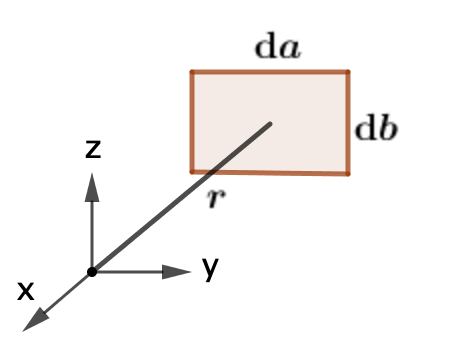
\includegraphics[width=.3\textwidth]{imagenes/imagenes23/T23IM03.png}
\end{figure}
\end{multicols}

Por definición, el ángulo sólido es adimensional. Al igual que los ángulos planos se les asocia la unidad arbitraria \emph{radián}, el ángulo sólido se mide en \emph{estéreo radianes}, $\mathrm{srad }$.


\begin{multicols}{2}
Vamos a expresar en polares el ángulo sólido.

arco=ángulo $\times$ radio

$\dd a = r \sin \theta \dd \varphi$

$\dd b= r \dd \theta$
\begin{figure}[H]
	\centering
	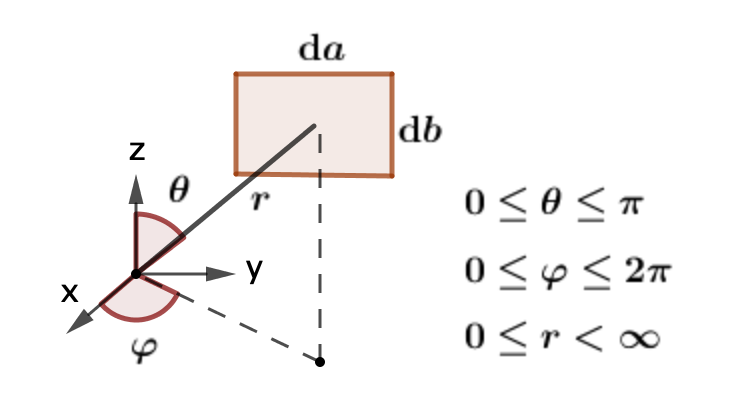
\includegraphics[width=.5\textwidth]{imagenes/imagenes23/T23IM04.png}
\end{figure}	
\end{multicols}

$$\boldsymbol{\dd \Omega=} \dfrac{\dd S}{r^2}=\dfrac{\dd a \ \dd b}{r^2}= \dfrac {r^2 \sin \theta \dd \varphi \dd \theta}{r^2} \boldsymbol{=\sin \theta \  \dd \theta \ \dd \varphi}$$

Nos interesa el ángulo sólido finito subtendido por una superficie finita, integrando:

$\Omega= \displaystyle \int_S \dfrac{\dd S}{r^2}=\int_{\varphi_1}^{\varphi_2} \dd \varphi \cdot \int_{\theta_1}^{\theta_2} \sin \theta \dd \theta = -(\varphi_2-\varphi_1)\cdot (\cos \theta_2-\cos \theta_1)$

Vamos a estudiar el caso particular del cálculo del \emph{ángulo solido subtendido por una superficie tridimensional cerrada} desde un punto interior y desde uno exterior a la misma.

\begin{enumerate}
\item 	 \emph{ángulo solido subtendido por una superficie tridimensional cerrada desde un punto interior a la misma.}

$0\leq \varphi\leq 2\pi;\ \  0\leq \theta\leq \pi \ \ \to \ \  \boldsymbol{\Omega=}-(2\pi-0)(\cos \pi -\cos 0) \boldsymbol{= 4\pi}  \mathrm{srad}$

Una superficie cerrada $S$, con un punto $\mathcal O$ interior, subtiende un ángulo sólido de $4\pi\ \mathrm{srad}$, independientemente de las características geométricas de $S$.

\begin{figure}[H]
	\centering
	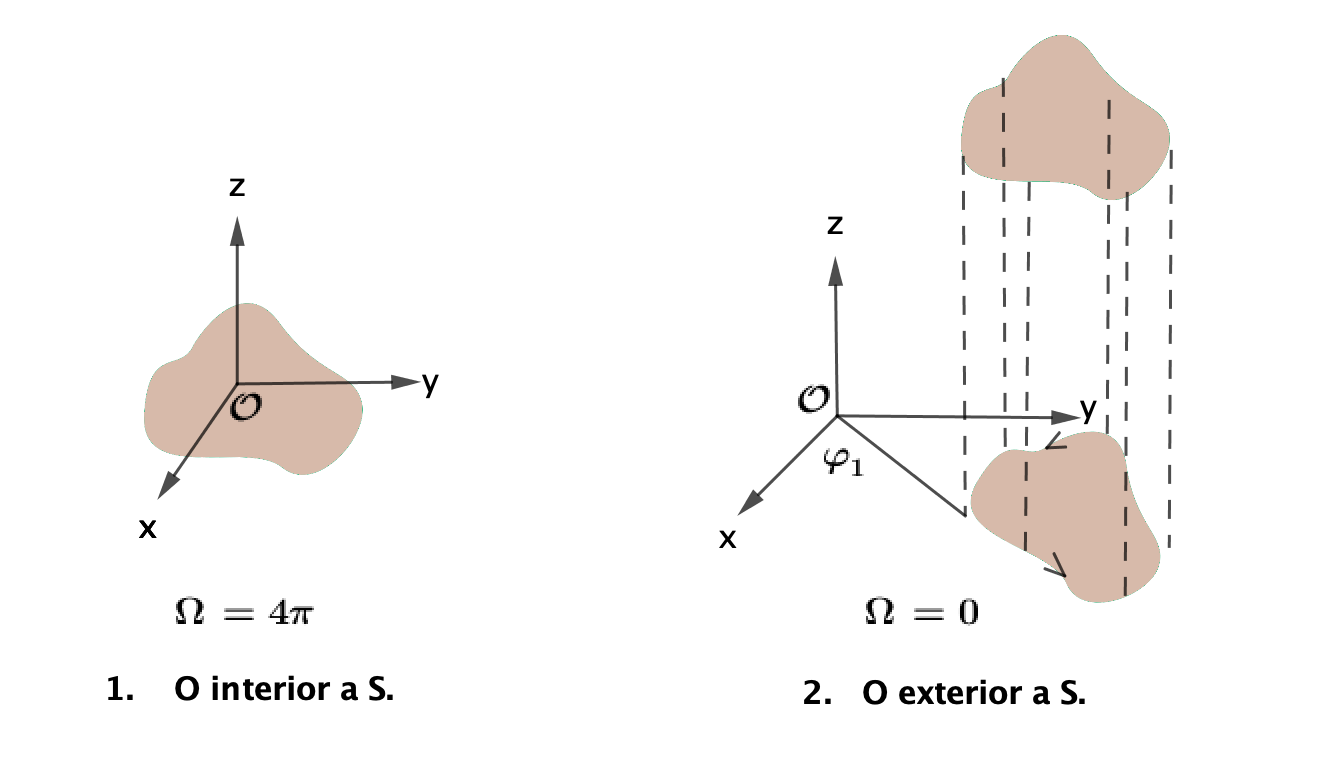
\includegraphics[width=1\textwidth]{imagenes/imagenes23/T23IM05.png}
\end{figure}

\item  \emph{ángulo solido subtendido por una superficie tridimensional cerrada desde un punto exterior a la misma.}

Para la proyección como curva cerrada de $S$ sobre el plano $XY$, el ángulo $\varphi=0$, no le da la vuelta al eje $Z$. Por lo que, $\ \boldsymbol{\Omega =0 \ \mathrm{srad}}$ 

Una superficie cerrada $S$, con un punto $\mathcal O$ exterior, subtiende un ángulo sólido de $0\ \mathrm{srad}$, independientemente de las características geométricas de $S$.
\end{enumerate}

\section{Ley de Gauss para el campo eléctrico}

Distribución continua de carga: $\displaystyle \ \vec E=\dfrac 1{4\pi \varepsilon_0} \int_\tau \dfrac{\rho \dd \tau}{r^2} \ \vec u_r$

Una carga puntual $q$ creará un campo eléctrico $\vec E$ y vamos a calcular el flujo que crea esta carga a atravesar una superficie cerrada $S$ en dos casos: a) $q$ es externa a $S$, y b) $q$ es interna a $S$.

\begin{figure}[H]
	\centering
	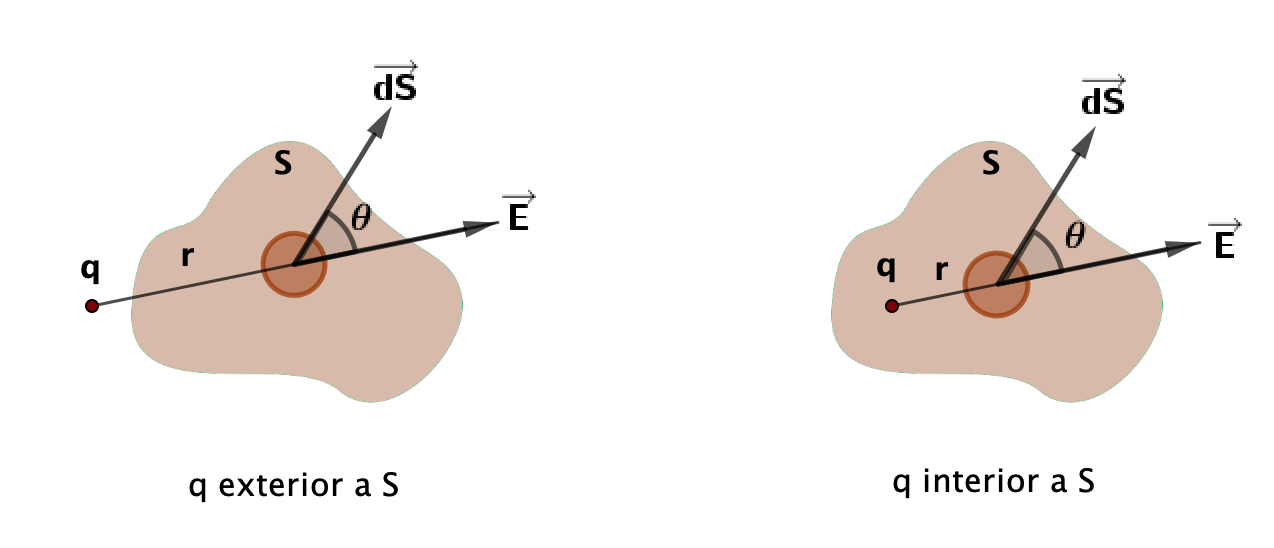
\includegraphics[width=1\textwidth]{imagenes/imagenes23/T23IM06.png}
\end{figure}

El flujo eléctrico elemental del campo que crea $q$ al atravesar $S$ es:

$\boldsymbol{ \dd \Phi_E=}\vec E \cdot \dd \vec S =E\cos \theta \dd S=\dfrac {q}{4\pi \varepsilon_0 r^2} \cos \theta \dd S= \dfrac {q}{4\pi \varepsilon_0} \dfrac {\cos \theta \dd S}{r^2} \boldsymbol{= \dfrac {q}{4\pi \varepsilon_0} \dd \Omega}$

Considerando $q=cte$ e integrando en toda la superficie cerrada,

$\displaystyle \subrayado{ \ \Phi_E= \ } \oint_S \vec E \cdot \dd \vec S= \dfrac {q}{4\pi \varepsilon_0} \oint_S \dd \Omega = \dfrac {q}{4\pi \varepsilon_0} \Omega = \begin{cases}
\subrayado{ \  \dfrac q {\varepsilon_0} \ \ \text{	si } q \text{ interior } S \ }\\
 \subrayado{\  0 \ \ \ \  \text{	si } q \text{ exterior} \ }S 
 \end{cases}$

Que es el \emph{Teorema de Gauss de la electrostática en el caso de una carga puntual}.

A partir de este resultado podemos generalizar para un sistema discreto de cargas:

$$\boldsymbol{ \Phi_E=} \displaystyle \oint_S \vec E_{total} \cdot \dd \vec S \boldsymbol{= \dfrac 1 {\varepsilon_0} \sum_{i=1}^N q_i}$$

\begin{multicols}{2}
donde $i=1,\cdots , N$ son las cargas \textbf{interiores} a la superficie, las cargas externas no interviene a nivel de flujo eléctrico. Esto constituye el \emph{Teorema de Gauss de la electrostática para el caso de una distribución discreta de cargas}.

\begin{figure}[H]
	\centering
	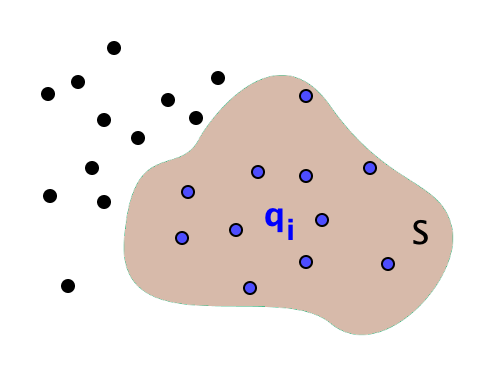
\includegraphics[width=.35\textwidth]{imagenes/imagenes23/T23IM07.png}
\end{figure}
\end{multicols}

Si lo que tenemos es una distribución continua $\rho$ de cargas, el flujo es

$$\displaystyle \displaystyle{ \Phi_E=} \oint_S \vec E \cdot \dd \vec S=\dfrac 1 {\varepsilon_0} \int_\tau \dd q \boldsymbol{ = \dfrac 1 {\varepsilon_0} \int_\tau \rho \dd \tau}$$

donde $\tau$ es el volumen que contiene a  las cargas interiores a la superficie cerrada $S$.
Esto constituye el \emph{Teorema de Gauss de la electrostática para el caso de una distribución continua de cargas}.

\section{Ejemplos del teorema de Gauss}

\begin{miparrafodestacado}

Como se mencionó, la ley de Gauss es útil para determinar campos eléctricos cuando la distribución de carga está caracterizada por un alto grado de simetría.  

Las superficies gaussianas no son reales.  La superficie gaussiana es una superficie imaginaria que se elige para satisfacer las condiciones mencionadas en este caso. No tiene que coincidir con una superficie física en una situación determinada. 

Al seleccionar la superficie, siempre debe aprovechar la simetría de la distribución de la carga de manera que $E$ pueda salir de la integral. El objetivo en este tipo de cálculo es encontrar una superficie para la que cada parte de la superficie satisfaga una o más de las condiciones siguientes: 

1. Demostrar por simetría que el valor del campo eléctrico es constante sobre la porción de superficie.
 
2. Que el producto escalar $\vec E \cdot \dd \vec S$ se expresa como un producto algebraico simple $E \dd S$, porque sean paralelos entre sí. 

3. Que el producto escalar sea cero, ya que $E$ y $\dd S$ son  perpendiculares entre sí.
 
4. Que el campo eléctrico es iguala cero sobre la porción de superficie. 

Diferentes porciones de la superficie gaussiana puedan satisfacen varias condiciones en tanto que cada porción satisfaga al menos una condición.  Si la distribución de carga no tiene simetría suficiente para que una superficie gaussiana que satisfaga estas condiciones se pueda encontrar, la ley de Gauss sigue siendo cierta,  pero no es útil para determinar el campo eléctrico para esta distribución de carga. 	
\end{miparrafodestacado}


\subsection{Campo eléctrico credo por una carga distribuida uniformemente sobre un plano}

$$\displaystyle \displaystyle{ \Phi_E=} \oint_S \vec E \cdot \dd \vec S{ = \dfrac 1 {\varepsilon_0} \int_\tau \rho \dd \tau =\dfrac {Q}{\varepsilon_0}}$$

\begin{figure}[H]
	\centering
	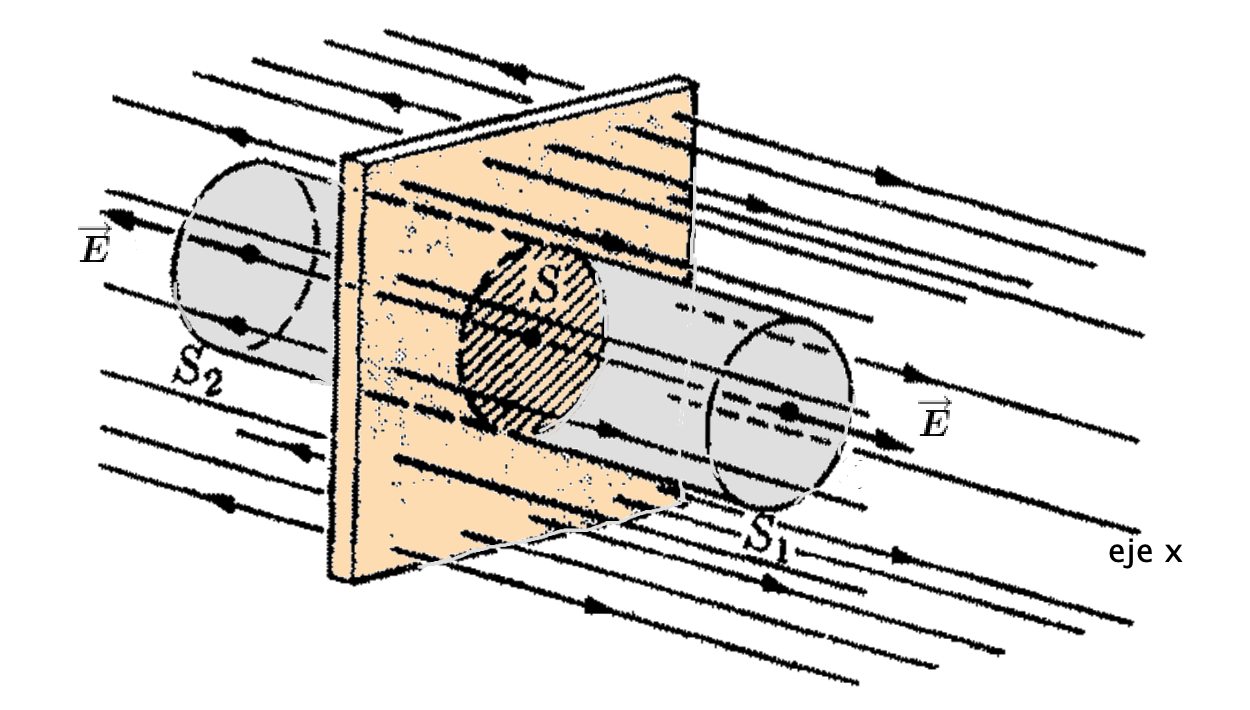
\includegraphics[width=1\textwidth]{imagenes/imagenes23/T23IM08.png}
\end{figure}

El campo elecétrico $\vec E$ es perpendicular al plano, si no fuese así habrían componentes tangenciales que provocarían un movimiento de las cargas y la distribución no sería uniforme.

El cilindro en gris define la superficie gaussiana (cerrada) que tomamos para aplicar el teorema de Gauss. A través de la superficie lateral del cilindro, el flujo es nulo ya que $\vec E \ \bot \ \dd \vec S$. Consecuentemente, el único flujo de líneas del campo que puede entras o salir de la superficie gaussiana es el que entre o salga por sus bases.

$\displaystyle \oint_S \vec E \cdot \dd \vec S= \int_S{S_1}  \vec E \cdot \dd \vec S +  \int_S{S_2}  \vec E \cdot \dd \vec + \cancelto{0}{\int_S{S_{lateral}}  \vec E \cdot \dd \vec S} = \vec E \cdot \vec S_1+\vec E \cdot \vec S_2 $

$\sigma=\dfrac Q S$, densidad superficial de carga en la placa.

Como $S_1=S_2 \ \to \ 2 E \cancel{S}=\dfrac 1{\varepsilon_0}Q_{int}= \dfrac 1 {\varepsilon_0} \sigma \cancel{S} \ \to $

$$ \subrayado{ \ \boldsymbol{E\ = \ \dfrac {\sigma}{2\varepsilon}} \ } $$

\emph{El campo eléctrico creado por una distribución continua de carga distribuida uniformemente sobre un plano es independiente de la distancia al plano, solo depende de la distribución de cargas.}

\subsection{Campo eléctrico producido por dos planos paralelos cargados con cargas iguales y opuestas}

\begin{figure}[H]
	\centering
	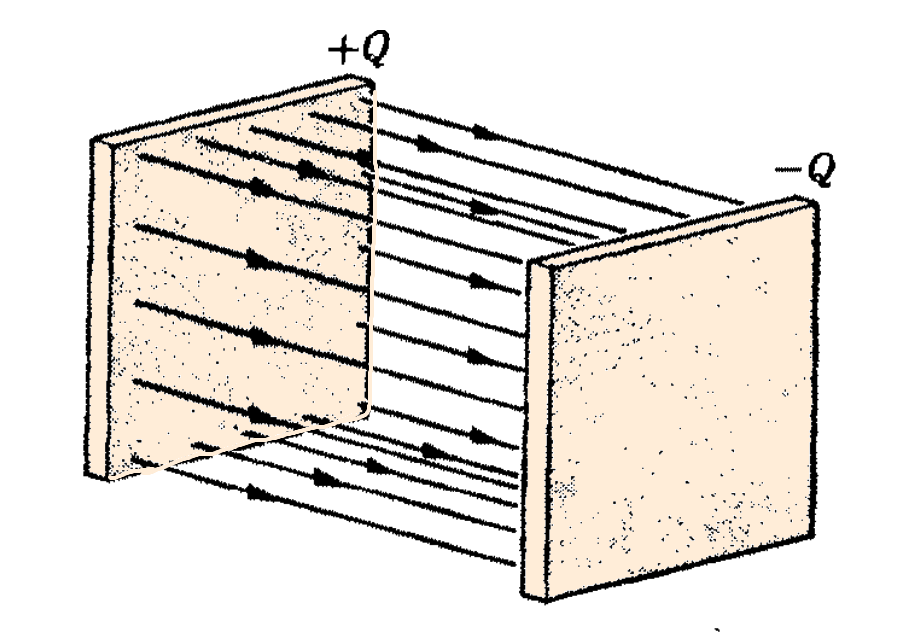
\includegraphics[width=.8\textwidth]{imagenes/imagenes23/T23IM09.png}
\end{figure}

$Q=\sigma S$

A la derecha de las placas: $\ E=\dfrac{\sigma+}{2\varepsilon_0}+\dfrac{\sigma-}{2\varepsilon_0}=\dfrac{+\sigma}{2\varepsilon_0}+\dfrac{-\sigma}{2\varepsilon_0}=0$.

 A la izquierda de las placas: $\ E=-\dfrac{\sigma+}{2\varepsilon_0}-\dfrac{\sigma-}{2\varepsilon_0}=-\dfrac{+\sigma}{2\varepsilon_0}-\dfrac{-\sigma}{2\varepsilon_0}=0$.

Entre las placas: $\ \dfrac{\sigma+}{2\varepsilon_0}-\dfrac{\sigma-}{2\varepsilon_0}=\dfrac{+\sigma}{2\varepsilon_0}-\dfrac{-\sigma}{2\varepsilon_0}=\dfrac{2\sigma}{2\varepsilon_0}=\dfrac{\sigma}{\varepsilon_0}$

\emph{El campo eléctrico entre dos placas  planoparalelas cargadas con cargas de distinto signo es constante, independiente de la distancia a las placas. Fuera de la zona entre las placas, el campo es nulo.}

\subsection{Campo eléctrico creado por una distribución esférica de cargas}

\begin{figure}[H]
	\centering
	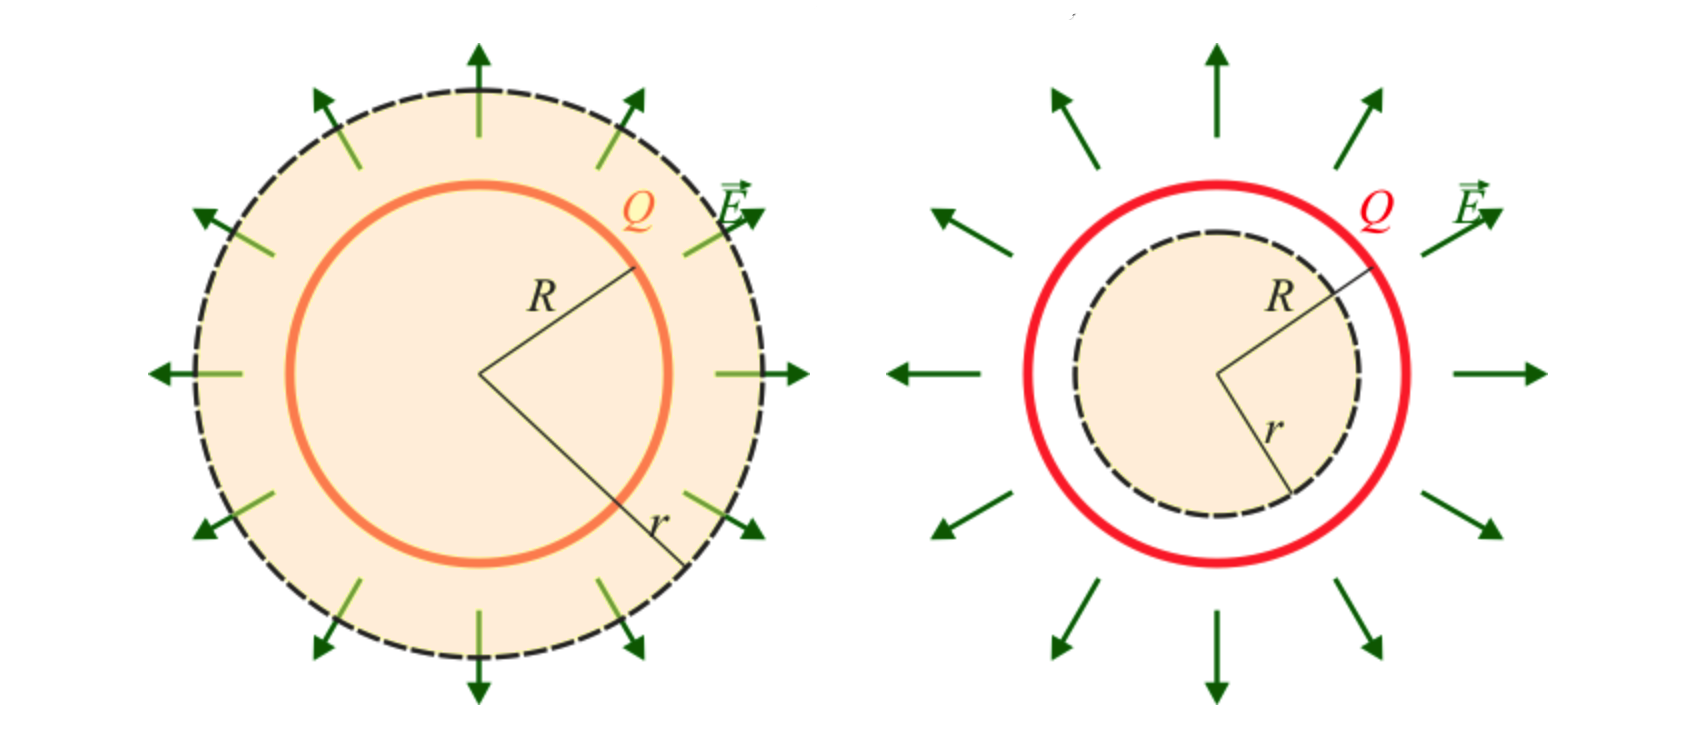
\includegraphics[width=1\textwidth]{imagenes/imagenes23/T23IM10.png}
\end{figure}

El campo eléctrica de una esfera cargada tiene simetría radial. Las superficies gaussianas que vamos a escoger van a ser esferas concéntricas de radios $r$ mayor y menor que el radio $R$ de la esfera cargada, por ello, $\vec E \ || \ \dd \vec S$ y $E=cte$ en todos los puntos de la superficie esférica.

\begin{itemize}
\item $\vec E$ para distancias $r>R$	

$\displaystyle \Phi_E= \oint_S \vec E \cdot \dd \vec S=\oint_S E \dd S=E\oint_S \dd S= E \ 4\pi r^2 = \dfrac {Q}{\varepsilon_0}$ 

Por lo que,

$$\subrayado{\  E(r>R)=\dfrac Q {4\pi \varepsilon_o r^2} \ }$$

\emph{El campo eléctrico creado por una distribución continua de carga en una esfera, para puntos externos $r>a$, es el mismo que produciría una carga puntual $Q$ igual a toda la carga de la esfera y situada en su centro.}

\item $\vec E$ para distancias $r<R$	

Hemos de distinguir entre dos posibilidades: que la carga de la esfera está distribuida solamente en su superficie o que lo esté en todo su volumen.

	\begin{itemize}
	\item $Q$ sobre la superficie esférica $4\pi R^2$, no hay carga en el interior de la esfera, solo está en su superficie (esto ocurre en los metales).
	
	$$ \subrayado{E(r<R)=0} \quad \subrayado{\ \text{distribución superficial de carga} \ }$$
	
	\emph{El campo eléctrico de una distribución superficial esférica de cargas en el interior de la esfera es nulo. No hay cargas en su interior.}
	
	\item $Q$ sobre todo el volumen $\frac 4 3 \pi R^3$ de la esfera. $\rho=cte=\dfrac Q{\frac 4 3 \pi R^3}$. Para $r<R$,
	
	$\displaystyle \Phi_E= \dfrac {Q_{r}}{\varepsilon_0}=\dfrac{\frac 4 3 \pi r^3 \rho}{\varepsilon_0}=\dfrac 4 3 \dfrac {\pi r^3 \rho}{\varepsilon_0}$
	
	$\displaystyle \Phi_E=\oint_S \vec E \cdot \dd \vec S= \oint E \dd S = E \oint_S \dd S= E\ 4\pi r^2$
	
	Por lo que,
	
	$$ \subrayado{ \ E=\dfrac{\rho r}{3\varepsilon_0}  \ } \quad \subrayado{ \ \text{distribución de carga en el volumen} \ }$$
	\end{itemize}
	
	\emph{El campo eléctrico de una distribución volumétrica  esférica de cargas en el interior de la esfera es directamente proporcional a $r$. Para $r=a \ \to \ E=\dfrac{\rho a}{3\varepsilon_0}$}.
\end{itemize}



\section{Forma diferencial de la ley de Gauss}

.


\begin{multicols}{2}
Vamos a encontrar una relación local, de punto, entre el campo eléctrico y la distribución de carga.

$\dd \tau=\dd x\ \dd y \ \dd z$

$\vec E$ en el centro de simetría de la figura.

Vamos a calcular el flujo eléctrico a través de todas las caras del elemento de volumen del cubo.
 
\begin{figure}[H]
	\centering
	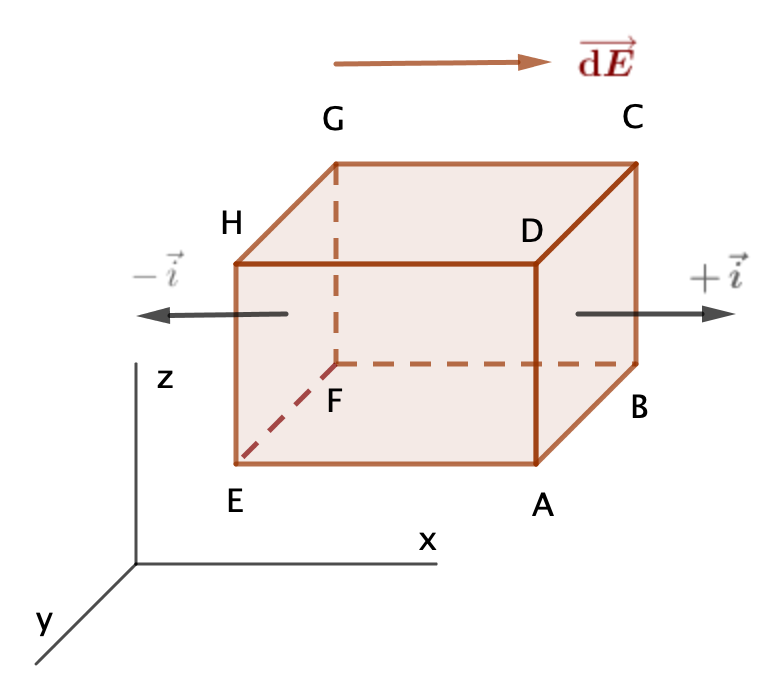
\includegraphics[width=.5\textwidth]{imagenes/imagenes23/T23IM11.png}
\end{figure}	
\end{multicols}

Entre los puntos $E$ y $A$ hay una variación del campo $\dd \vec E$

------ Cara $ABCD$: el campo vale $\ \vec E + \dfrac 1 2 \dd \vec E$

$\dd \Phi_{ABCD}=\left( \vec E + \dfrac 1 2 \dd \vec E \right) \cdot \vec i \ \dd y \dd z=E_x \ \dd y \dd z + \dfrac 1 2 \dd E_x \ \dd y \dd z$ 

En el caso de campos electrostáticos en que estamos, el campo puede variar con la distancia, pero no con el tiempo, $\ E=E(x,y,z)$.

$\displaystyle \dd E_x=\pdv{E_x}{x} \dd x+\pdv{E_x}{y} \dd y+\pdv{E_x}{z} \dd z$

Como, nos hemos desplazado en el eje $x$ desde el centro del elemento de volumen, solo hay variación en $\dd x$, y $\dd y=\dd z=0$, por lo que: 

$\displaystyle \dd E_x=\pdv{E_x}{x} \dd x \quad \to \quad$

$\displaystyle \dd \Phi_{ABCD}=
E_x \ \dd y \dd z + \dfrac 1 2 \dd E_x \ \dd y \dd z=
E_x \ \dd y \dd z + \dfrac 1 2 \pdv{E_x}{x} \ \dd x \dd y \dd z$

Análogamente: $\ \dd \displaystyle \Phi_{EFGH}= \left( \vec E - \dfrac 1 2  \dd \vec E \right) \cdot (-\vec i) \ \dd y \dd z= 
-E_x \ \dd y \dd z + \dfrac 1 2 \pdv{E_x}{x} \ \dd x \dd y \dd z$

$\displaystyle \dd \Phi_x= \dd \Phi_{ABCD}+\dd \Phi_{CDEF}= \pdv{E_x}{x}\ \dd x \dd y \dd z=\pdv{E_x}{x} \ \dd \tau$

Mediante razonamientos análogos, $\ \displaystyle \dd \Phi_y=\pdv{E_y}{y} \ \dd \tau;\quad \displaystyle \dd \Phi_z=\pdv{E_z}{z} \ \dd \tau$

Por lo que, $\ \displaystyle \dd \Phi=\dd \Phi_x+\dd \Phi_y+\dd \Phi_z=\left( \pdv{E_x}{x}+\pdv{E_y}{y}+\pdv{E_z}{z} \right) \ \dd \tau$

Como la ley de Gauss dice: $\quad \dd \Phi_E=\dfrac 1 {\varepsilon_0} \rho \dd \tau$, finalmente tenemos que

\begin{equation}
\label{Gauss-diferencial}
\subrayado{ \ \boldsymbol { \left( \pdv{E_x}{x}+\pdv{E_y}{y}+\pdv{E_z}{z} \right)\  =\ \dfrac {\rho}{\varepsilon_0}   }	 \ }
\end{equation}

\emph{Ley de Gauss en forma diferencial}, es una ecuación local o de punta, da cuenta de la variación del campo en función de la densidad de carga en el punto $(x,y,z)$.

Teniendo en cuenta el \emph{operador nabla}, podemos escribir la \textbf{ley de Gauss en forma diferencial} como:

\begin{equation}
\label{Gauss-diferencial2}
\subrayado{\  \boxed { \ \boldsymbol { \overrightarrow{\grad} \cdot \overrightarrow{E} \  =\ \dfrac {\rho}{\varepsilon_0}  } \ } \ }  \qquad \textbf{Divergencia del campo eléctrico.}
\end{equation}

\section{Ecuaciones de Poisson y de Laplace}

Son simples consecuencias del teorema de Gauss.

\subsection{Ecuación de Gauss}

$\vec E$ conservativo $\to \vec E=-\vec{\grad} V; \ V$ es el \textbf{potencial eléctrico} (escalar)

$\vec {\grad} \cdot \vec E= \vec {\grad} (-\vec{\grad} V)=\dfrac \rho {\varepsilon_0} \quad \to \quad \vec {\grad} \cdot ( \vec {\grad} V )=-\dfrac \rho {\varepsilon_0}$

$\displaystyle \vec {\grad} \cdot  \vec {\grad}=
\left( \vec i \pdv{x} +\vec j \pdv{y} +\vec k \pdv{z} \right) \cdot
\left( \vec i \pdv{x} +\vec j \pdv{y} +\vec k \pdv{z} \right)=$

$\displaystyle = \pdv[2]{x}+\pdv[2]{y}+\pdv[2]{z}=\grad^2=\nabla \quad \to \quad \displaystyle \vec {\grad} \cdot  \vec {\grad}=\nabla $

\begin{equation}
\label{Ec-Poisson}
\subrayado{\ \boxed{\ \boldsymbol{\grad^2 V=-\dfrac \rho {\varepsilon_0}} \ } \ } \qquad \textbf{Ecuación de Poisson}	
\end{equation}

\emph{La ecuación de Poisson es una relación local entre el potencial eléctrico y la densidad de carga}

\subsection{Ecuación de Laplace}

En los puntos donde no hay carga,

\begin{equation}
\label{Ec-Laplace}
\subrayado{\ \boxed{\ \boldsymbol{\rho=0 \ \ \to \ \  \grad^2 V=0 } \ } \ } \qquad \textbf{Ecuación de Laplace}	
\end{equation}

\begin{ejem}
Calculo del potencial eléctrico y el campo eléctrico en la región vacía comprendida entre dos planos paralelos, cargados a los potenciales $V_1$ y $V_2$	
\end{ejem}

\begin{multicols}{2}
No hay carga entre las placas: 

$\rho=0 \to $ Laplace $\to \grad^2V=0$

La simetría del problema nos induce a pensar el el campo solo tiene componente $x$, por lo que

$\displaystyle \dv[2]{V}{x}=0 \ \to \ \dv{V}{x}=cte$

Físicamente, $\displaystyle \dv{V}{x}=-E$, 

luego $E=cte$ . Integrando:
\begin{figure}[H]
	\centering
	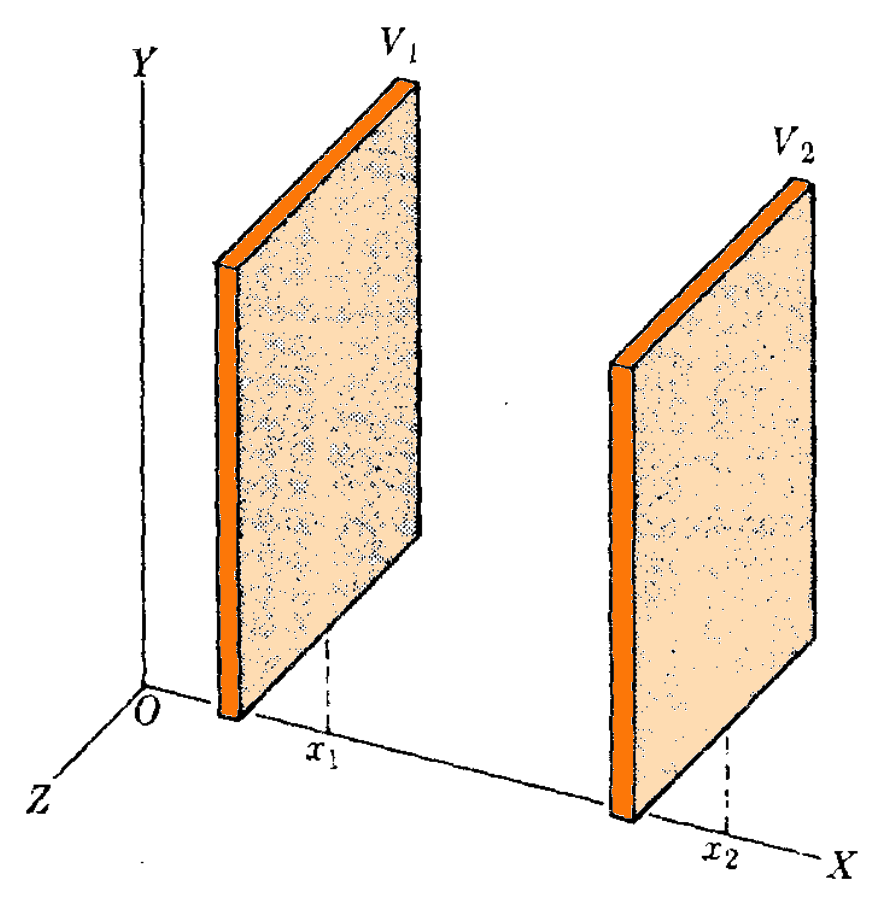
\includegraphics[width=.5\textwidth]{imagenes/imagenes23/T23IM12.png}
\end{figure}	
\end{multicols}

$\displaystyle \int_{V_1}V \dd V=-E \int_{x_1}^x \dd x \ \to \ V-V_1=-E(x-x_1)$

$$V_2=V_1-E(x_2-x_1); \qquad x_2-x_1=d \ \to \ 	E=-\dfrac {V_2-V_1}{d}$$

La dependencia analítica de $V$ en función de la distancia $x$ es la ecuación de una recta, es decir, el potencial eléctrico varía linealmente con la distancia. Resultado que concuerda con el obtenido en el capítulo anterior (subsección \ref{EV-Ecte}).

\begin{ejem}
Resolver el mismo problema anterior pero suponiendo que entre las placas hay una distribución uniforme de carga.
\end{ejem}

Ahora debemos aplicar la ecuación de Poisson. Por la simetría del problema, el potencial solo depende de $x$ y podremos escribir:

$\displaystyle \dv[2]{V}{x}=-\rho / \varepsilon_0$, con $\rho=cte$. Integrando,

$\displaystyle \int_{x_1}^x \dv[2]{V}{x} \dd x = -\dfrac 1 {\varepsilon_0} \int_{x_1}^x \rho \dd x = -\dfrac \rho {\varepsilon_0} \int_{x_1}^x \dd x$

$\displaystyle \dv{V}{x}-\cancelto{-E_1}{\left( \dv{V}{x} \right)_{x=x_1}}=-\dfrac \rho {\varepsilon_0} (x-x_1)$

$\displaystyle \cancelto{-E}{\dv{V}{x}}=-E_1-\dfrac \rho {\varepsilon_0} (x-x_1)$

$\displaystyle E=E_1+\dfrac \rho {\varepsilon_0} (x-x_1)$

El campo eléctrico varía linealmente con $x$. Integrando de nuevo,

$\displaystyle \int_{V_1}^V \dd V = -\int_{x_1}^x E_1 \dd x - \dfrac \rho {\varepsilon_0} \int_{x_1}^x (x-x_1) \dd x$

$V=V_1-E_1(x-x_1)-\dfrac \rho {2\varepsilon_0} (x-x_1)^2$

El potencial eléctrico varia con $x^2$.

Haciendo $x_2=x_1 \quad \to \quad V_2=V_1-E_1(x_2-x_1)-\dfrac \rho {2\varepsilon_0} (x_2-x_1)^2$, de donde se despeja $E$.





\section{Problemas}

\begin{prob}
Hallar el campo eléctrico creado por una distribución cilíndrica de carga de longitud infinita.	
\end{prob}

$C$, cilindro de radio $a$ y longitud $L$; $\lambda$ densidad `lineal' de carga, $\lambda=q/L$.

Por simetría, el campo eléctrico en un punto depende solo de la distancia al eje del cilindro y está dirigido radialmente.

\begin{figure}[H]
	\centering
	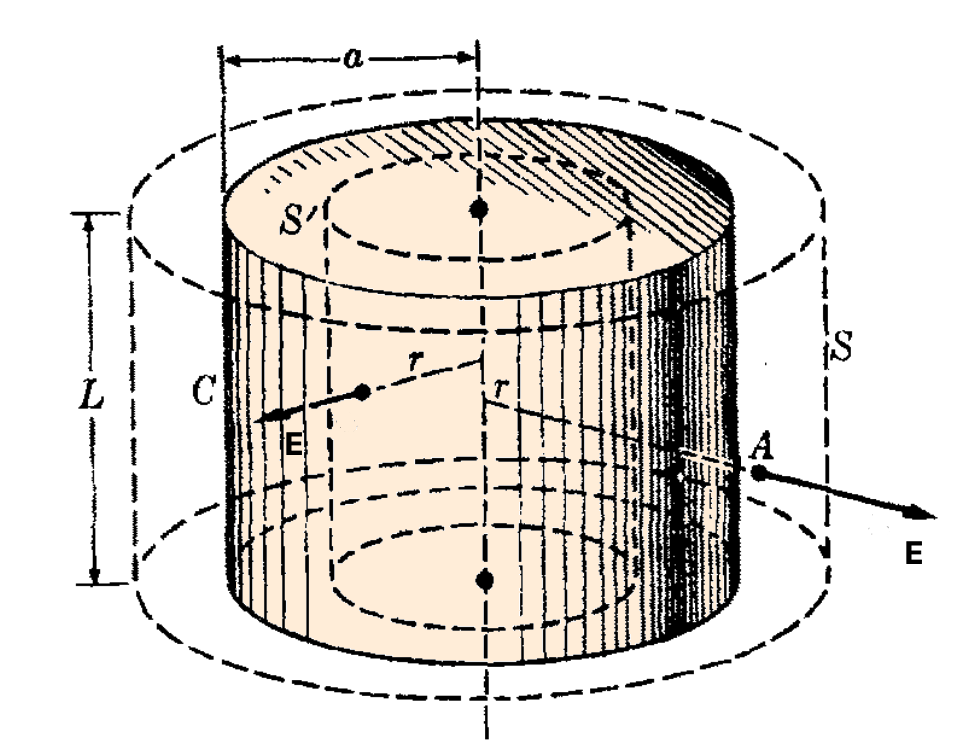
\includegraphics[width=.85\textwidth]{imagenes/imagenes23/T23IM14.png}
\end{figure}


Tomamos como superficie gaussiana una superficie $S$ cilíndrica de radio $r$ coaxial con el cilindro $C$. El flujo a través de esta superficie se compone del flujo a través de la superficie lateral y el flujo a través de sus dos bases, siendo estos últimos nulos pues $\vec E \ \bot \vec S_{base}$. Solo queda el flujo a través de la superficie lateral de $S:\quad S\Phi_E=2\pi r L E$

Aplicando el teorema de Gauss, tendremos:

\begin{itemize}
\item $r>a$

La carga es $q=\lambda L \quad \to Gauss: \qquad 2\pi rL E=\dfrac{\lambda L}{\varepsilon_0}$

$$E=\dfrac \lambda {2\pi \varepsilon_0 r}$$
\item $r<a$

Ahora, la superficie gaussiana es $S'$ el la figura.

	\begin{itemize}
	\item Carga distribuida superficialmente.
	
	No hay carga en el interior de $' \quad Gauss:\qquad 2\pi r L E=0$
	
	$$E=0$$
	\item Carga distribuida volumétricamente.
	
	La carga interior a la superficie $\ S' \ $ de radio $\ r<a\ $ es $\quad q'=\lambda L \dfrac {r^2}{a^2}; \quad Gauss: \qquad 2\pi r L E=q'$
	
	$$E=\dfrac{\lambda r}{2 \pi \varepsilon_0 a^2}$$
	\end{itemize}	
\end{itemize}

\vspace{10mm} %*****************************************
\begin{prob}
Hallar el flujo eléctrico y la densidad de carga	 en el interior de un cubo de lado $a$ colocado en na región en que el valor del campo es: $\ a) \vec E=\vec i\ cx^2; \quad b)\ \vec E=c(\vec i\ y+\vec j \ x)$
\end{prob}

$a)\qquad \displaystyle \dfrac {\rho}{\varepsilon_0}=\vec \grad \cdot \vec E=
\pdv{E_x}{x}+\cancelto{0}{\pdv{E_y}{y}}+\cancelto{0}{\pdv{E_z}{z}}=2cx \ \to \ \ \rho=2c\varepsilon_0 x$

$\phi_E= \displaystyle \oint \vec E \cdot \dd \vec S=\dfrac 1 {\varepsilon_0} \int_\tau \rho \dd \tau= =
\dfrac 1 {\varepsilon_0} \int_\tau \rho a^2 \dd x
 2ca^2 \int_0â x \dd x=\dfrac 2 3 c a^5$
 
 $b) \qquad  
\displaystyle \dfrac {\rho}{\varepsilon_0}=0=\vec \grad \cdot \vec E=
\cancelto{0}{\pdv{E_x}{x}}+\cancelto{0}{\pdv{E_y}{y}}+\cancelto{0} = 0 \ \to \ \ \rho=0 x$

$\vec E=cy \vec i + cx\ \vec j=E_x \vec i + E_y \vec j$

$\Phi_E=\displaystyle \oint \vec E \cdot \dd \vec S =\dfrac 1 {\varepsilon_0} \int_\tau \rho \dd \tau =0$

\vspace{10mm} %*****************************************
\begin{prob}
Un recipiente hemiesférico de radio $R$ tiene una carga total $q$	distribuida uniformemente en su superficie interior. Encontrar el campo eléctrico en el centro de curvatura.
\end{prob}

\begin{figure}[H]
	\centering
	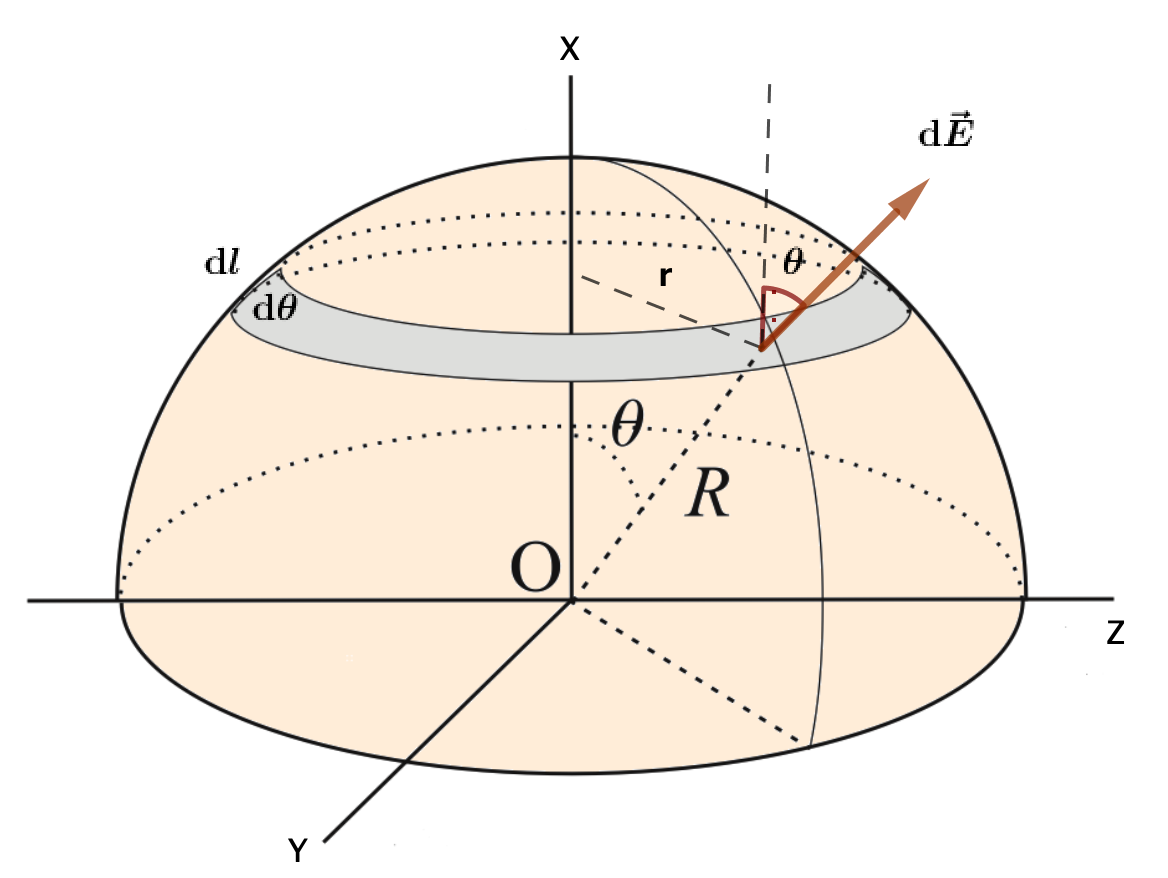
\includegraphics[width=.85\textwidth]{imagenes/imagenes23/T23IM15.png}
\end{figure}

$\dd E_x=\dd E \cos \theta = \dfrac {\sigma \dd S_{anillo}}{4\pi \varepsilon_0 R^2}\cos \theta$

$\dd S=2\pi r \dd l =2\pi R \sin \theta \ R\dd \theta=2\pi R^2 \sin \theta \dd \theta$

$\displaystyle \dd E_x=\dfrac{\sigma 2 \pi R^2 \sin \theta \cos \theta \dd \theta}{4\pi \varepsilon_0 R^2}=\dfrac{\sigma}{4\varepsilon_0} \int_0^{\pi/2}\sin 2 \theta \dd \theta$

\rightline{ \textbf{\textcolor{blue}{acábese}}}

\justify

\begin{prob}
Se dispone, en forma alternativa, un número infinito de cargas positivas y negativas de valor $q$ sobre una línea recta. La separación entre cargas adyacentes es siempre la misma, $r$. Determinar la energía potencial de una de estas cargas.	
\end{prob}

\begin{figure}[H]
	\centering
	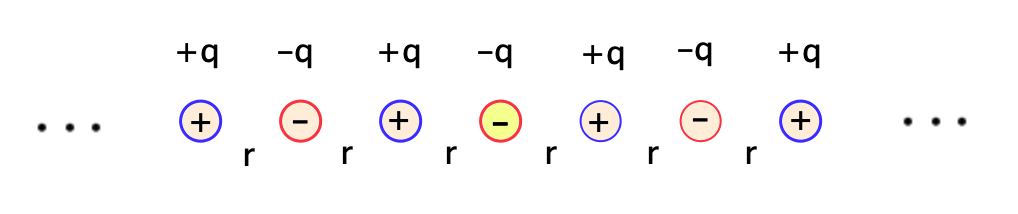
\includegraphics[width=1\textwidth]{imagenes/imagenes23/T23IM16.png}
\end{figure}

$V_r=\dfrac {q}{4\pi \varepsilon_0 r}+\dfrac {q}{4\pi \varepsilon_0 r}=\dfrac {q}{2\pi \varepsilon_0 r}$

$V_{2r}=-\dfrac {q}{4\pi \varepsilon_0 (2r)}-\dfrac {q}{4\pi \varepsilon_0 (2r)}=-\dfrac {q}{2\pi \varepsilon_0 (2r)}$

$V_{3r}=\dfrac {q}{4\pi \varepsilon_0 (3r)}+\dfrac {q}{4\pi \varepsilon_0 (3r)}=\dfrac {q}{2\pi \varepsilon_0 (3r)}$

etcétera

$V=\displaystyle \sum{i=1}^\infty v_{ir}=\dfrac {q}{2\pi \varepsilon_0 r}\sum_{i=1}^\infty
\left( 1-\dfrac 1 2 + \dfrac 1 3 - \dfrac 1 4 + \cdots \right)$

En el paréntesis aparece el desarrollo en serie de McLauirin de $\ln(1+x)$ en $x=1$, por lo que

$V=\dfrac {q}{2\pi \varepsilon_0 r} \ln 2 \quad \to \quad \mathcal E_p=-2 \dfrac {q}{4\pi \varepsilon_0 r} \ln 2 = - \dfrac {q^2}{4\pi \varepsilon_0 r}\ln 2$

\newpage %********************************************************
\begin{myblock}{?´Qué es a ley de Gauss?}

\begin{figure}[H]
	\centering
	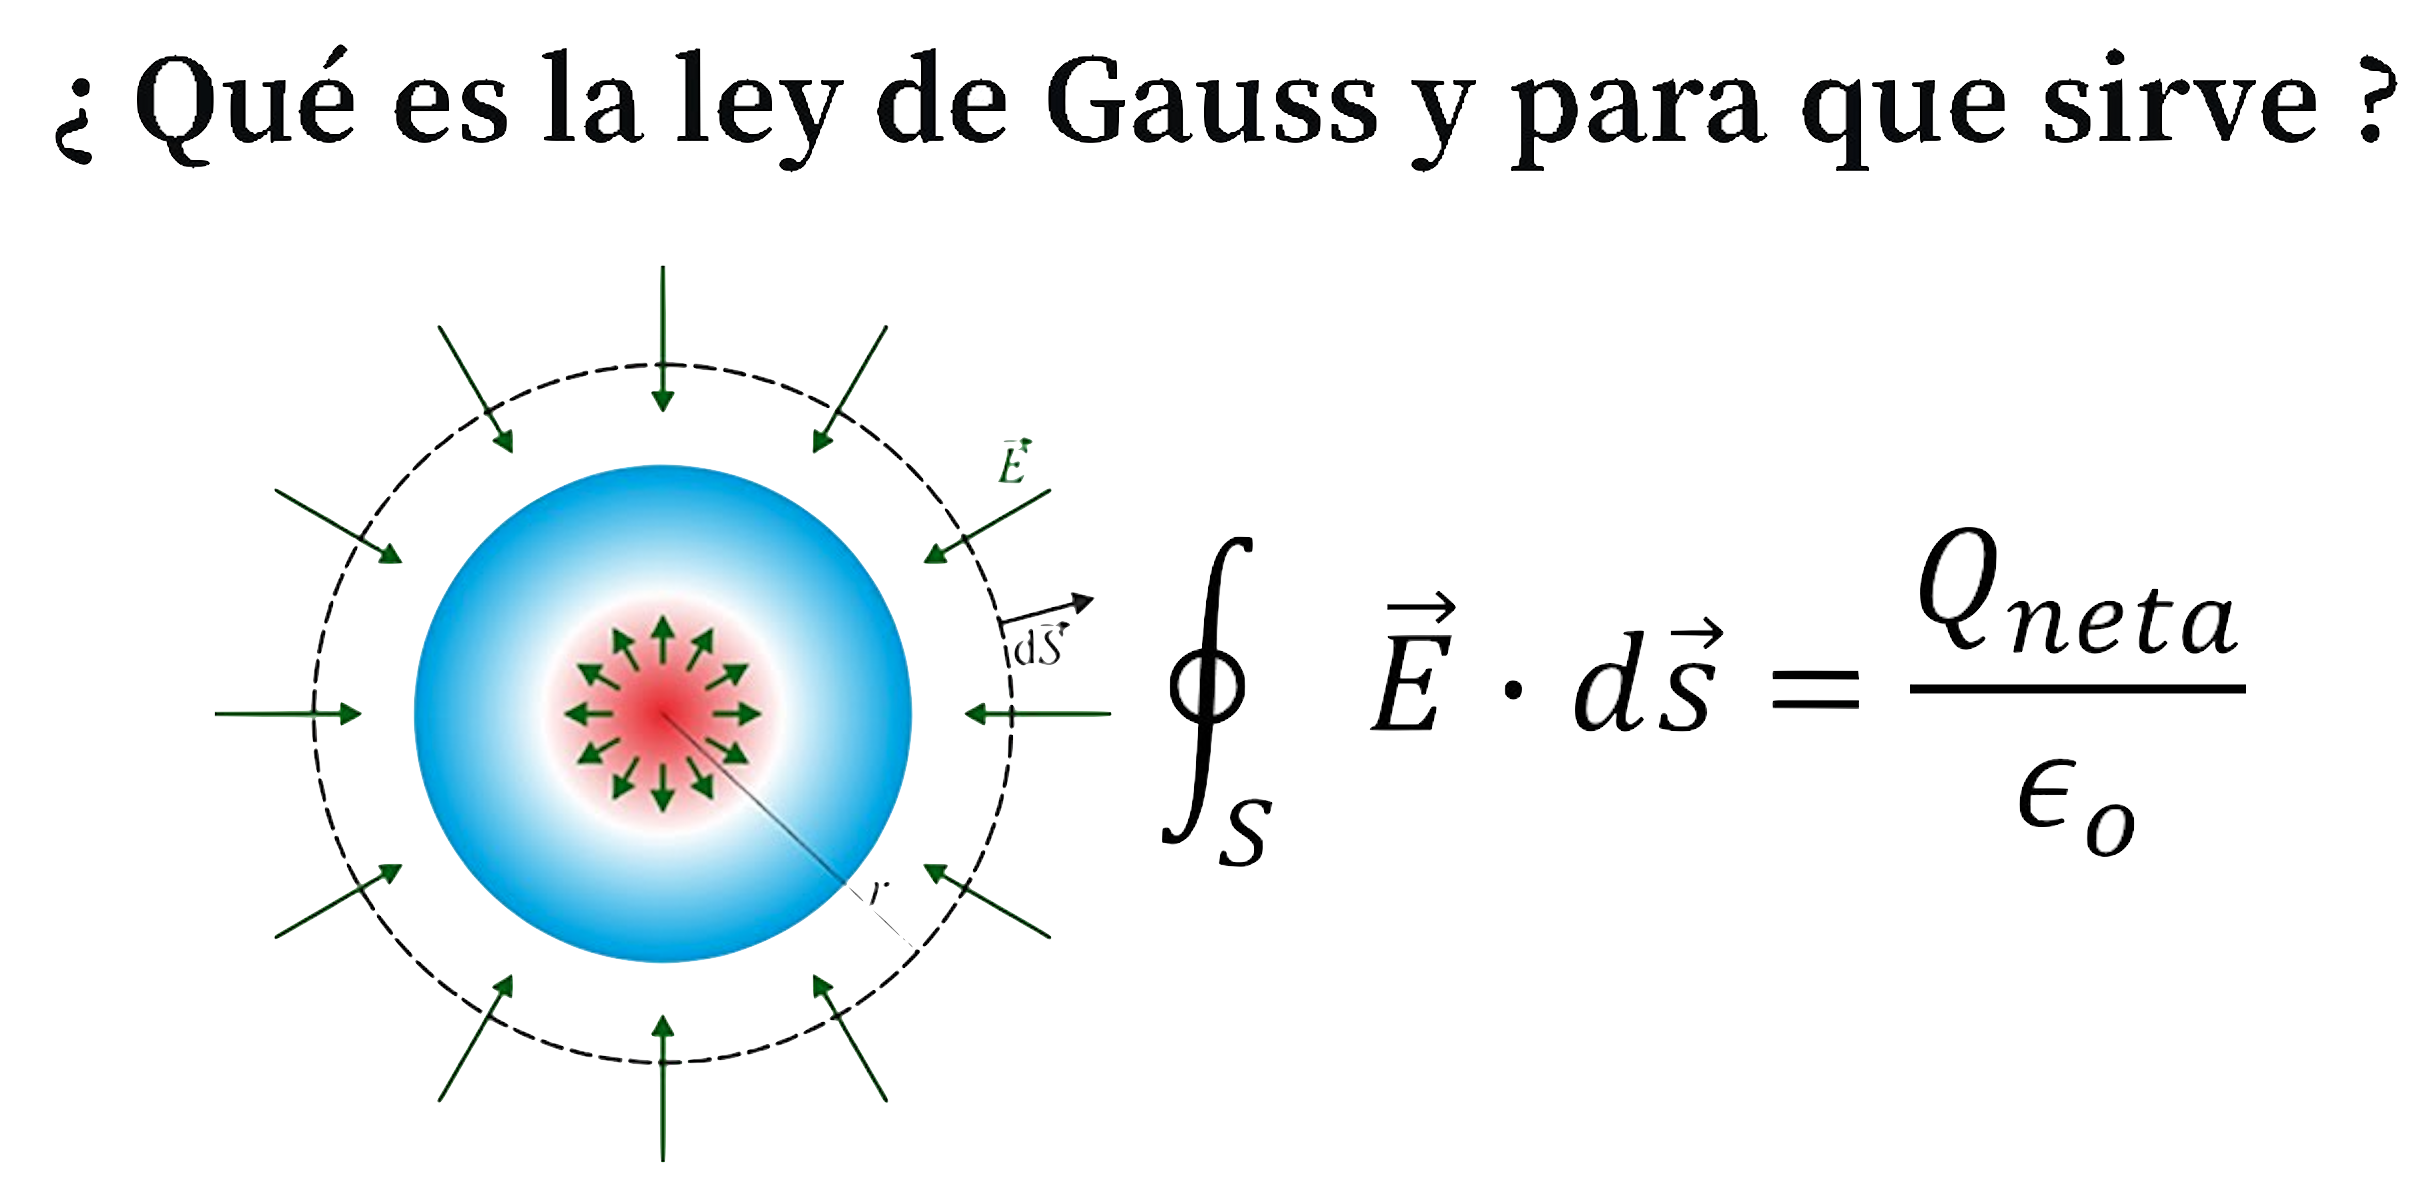
\includegraphics[width=.9\textwidth]{imagenes/imagenes23/T23IM13.png}
\end{figure}

\vspace{2mm} En física las propiedades de simetría de los sistemas constituyen una herramienta importante para simplificar los problemas. Muchos sistemas físicos tienen simetría: un cuerpo cilíndrico no se ve distinto después de hacerlo girar sobre su eje, y una esfera de metal con carga se ve igual una vez que se ha hecho girar alrededor de cualquier eje que pase por su centro. 

\vspace{2mm} La ley de Gauss trata de lo siguiente: dada cualquier distribución general de carga, se rodea con una superficie imaginaria que la encierre y luego se observa el campo eléctrico en distintos puntos de esa superficie imaginaria. Es una relación entre el campo en todos los puntos de la superficie y la carga total que ésta encierra .

\vspace{2mm} La ley de Gauss es parte de la clave para utilizar consideraciones de simetría que simplifiquen los cálculos del campo eléctrico. Pero la ley de Gauss es algo más que un método para hacer ciertos cálculos con facilidad. En realidad es un enunciado fundamental acerca de la relación que hay entre las cargas eléctricas y los campos eléctricos. Entre otras cosas, la ley de Gauss ayuda a entender cómo se distribuye la carga en los cuerpos conductores. 
\end{myblock}